\section{Risultati}


\begin{frame}{Esecuzione ideale}
	\begin{itemize}
		\item Inizialmente esecuzione simulata in ambiente ideale, tramite
		\texttt{statevector\_simulator}
		\begin{figure}
			\centering
			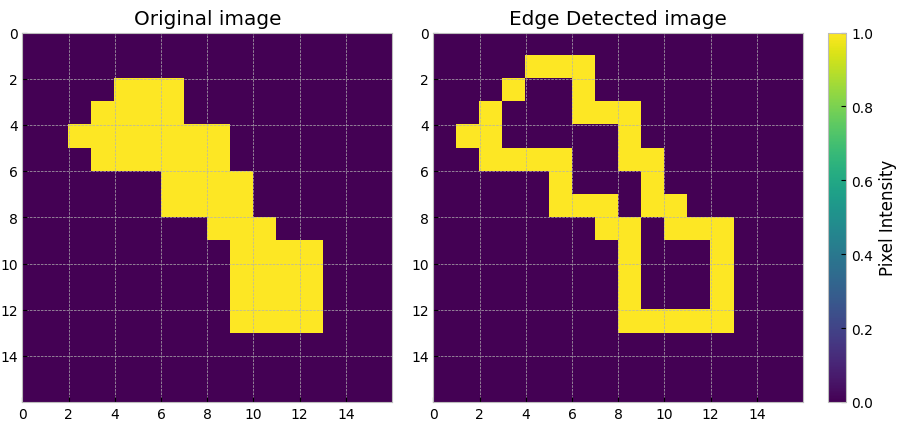
\includegraphics[width=0.9\textwidth]{statevector-detection.png}
		\end{figure}
	\end{itemize}
\end{frame}

\begin{frame}{Esecuzione con rumore}
	\begin{itemize}
		\item<1-> Successivamente è stato aggiunto il modello di rumore
		\item<2-> Generale miglioramento all'aumentare del numero di \emph{shots}
		\begin{figure}
			\centering
			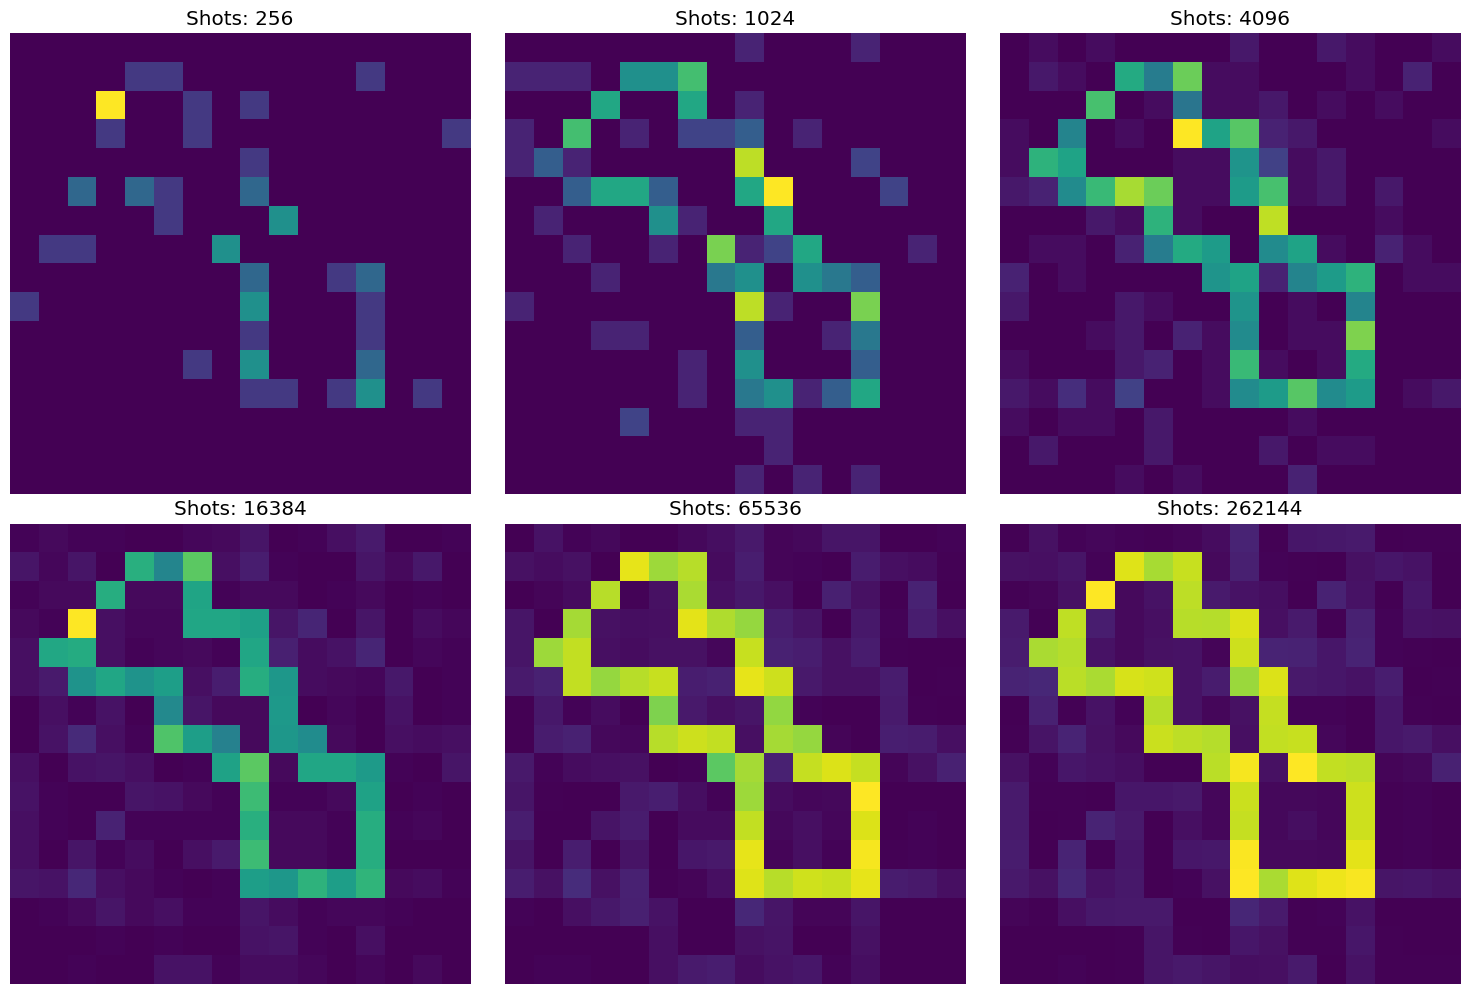
\includegraphics[width=0.8\textwidth]{16x16-shots.png}
		\end{figure}
	\end{itemize}
\end{frame}

\begin{frame}{Il \emph{transpiling}}
	\begin{itemize}
		\item \emph{Transpiling} oneroso, anche per immagini 4x4
		\item Per un'immagine 2x2, profondità del circuito risultante pari a 64
		\begin{figure}
			\centering
			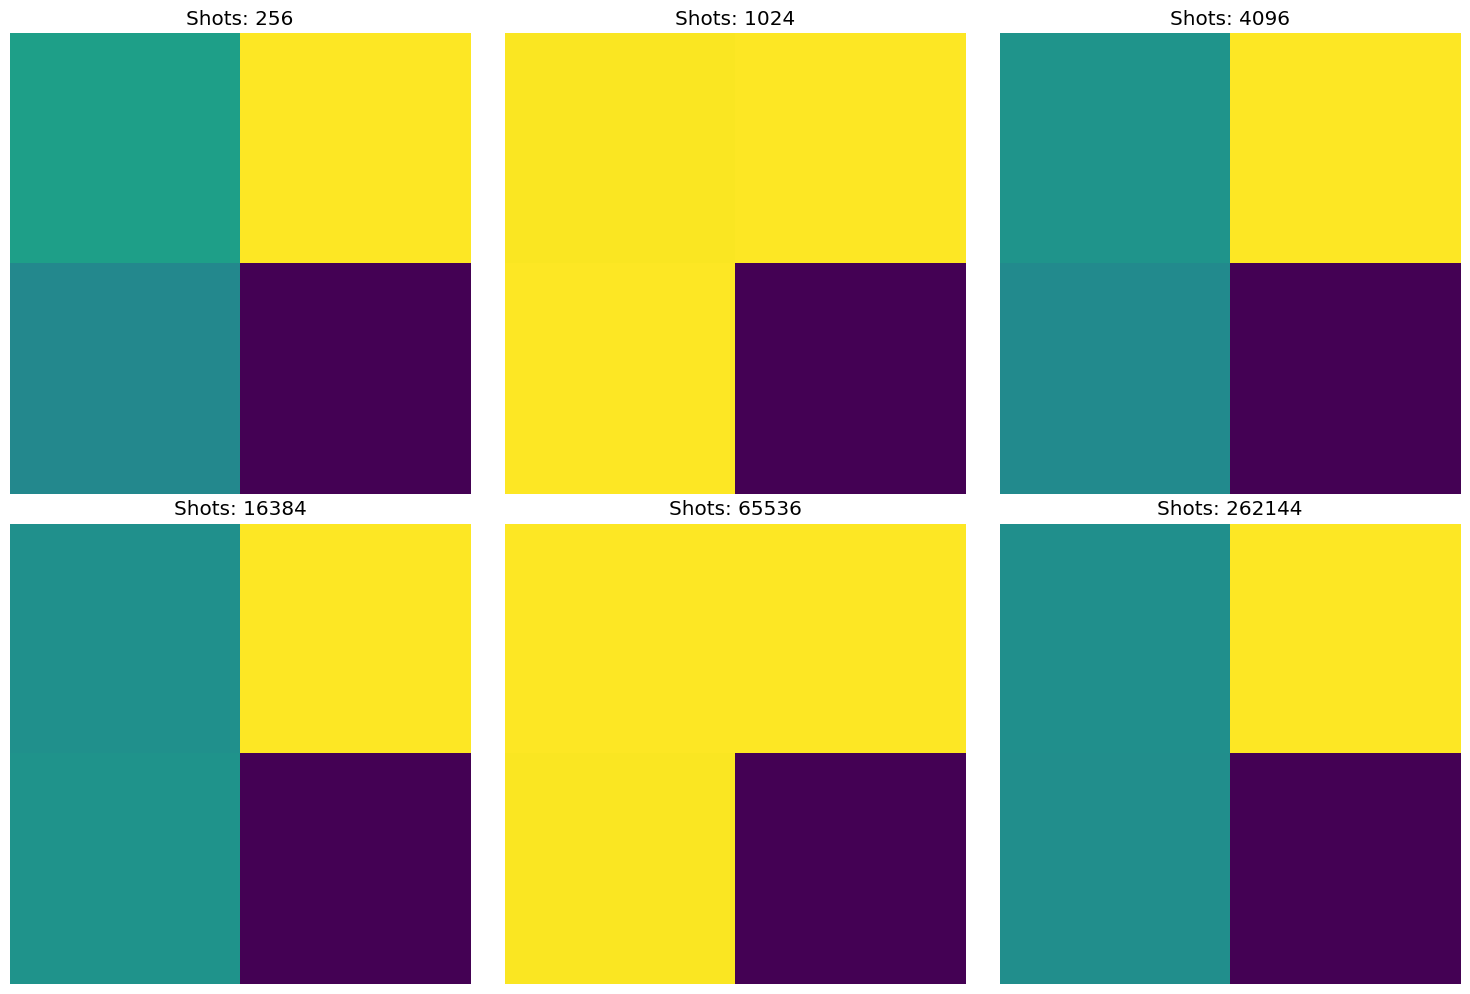
\includegraphics[width=0.7\textwidth]{2x2-shots.png}
			\caption{Simulazione con rumore con variazione sul numero di shots,
			immagine 2x2}
		\end{figure}
	\end{itemize}
\end{frame}

\begin{frame}{Complessità spaziale e computazionale}
	Sia $N=2^n,n \in \mathbb{N}$ la dimensione dell'immagine.
	\begin{table}[h]
		\centering
		\renewcommand{\arraystretch}{1.5}
		\begin{tabular}{|c|c|c|}
			\hline
			\rowcolor{gray!20}  % Imposta il colore di sfondo grigio chiaro
			\textbf{Algoritmo} & \textbf{Costo Spaziale} & \textbf{Costo Computazionale}\footnote{In riferimento al solo calcolo dei gradienti.} \\  
			\hline
			Classici & $\mathcal{O}(N=2^n)$ & $\mathcal{O}(N=2^n)$\\  
			\hline
			QSobel & $\mathcal{O}(2n+1)$ & $\mathcal{O}(n^2)$ \\  
			\hline
			\rowcolor{green!20}
			QHED & $\mathcal{O}(n+1)$ & $\mathcal{O}(1)$ \\  
			\hline
		\end{tabular}
		\caption{Confronto tra il costo spaziale e computazionale di diversi algoritmi}
		\label{tab:costo-spaziale-computazionale}
	\end{table}
\end{frame}
